\def\mytitle{Workbook}
\def\myauthor{}
\def\contact{40182161}
\def\mymodule{Fundamentals of Parallel Systems (SET09109)}

\documentclass[10pt, a4paper]{article}
\usepackage[a4paper,outer=1.5cm,inner=1.5cm,top=1.75cm,bottom=1.5cm]{geometry}
\onecolumn
\usepackage{graphicx}
\graphicspath{{./images/}}
%colour our links, remove weird boxes
\usepackage[colorlinks,linkcolor={black},citecolor={blue!80!black},urlcolor={blue!80!black}]{hyperref}
%Stop indentation on new paragraphs
\usepackage[parfill]{parskip}
%% all this is for Arial
\usepackage[english]{babel}
\usepackage[T1]{fontenc}
\usepackage{helvet}
\renewcommand{\familydefault}{\sfdefault}
%Napier logo top right
\usepackage{watermark}
%Lorem Ipusm dolor please don't leave any in you final repot ;)
\usepackage{lipsum}
\usepackage{xcolor}
\usepackage{listings}
%give us the Capital H that we all know and love
\usepackage{float}
%tone down the linespacing after section titles
\usepackage{titlesec}
%Cool maths printing
\usepackage{amsmath}
%PseudoCode
\usepackage{algorithm2e}
\usepackage{subfig}

\titlespacing{\subsection}{0pt}{\parskip}{-3pt}
\titlespacing{\subsubsection}{0pt}{\parskip}{-\parskip}
\titlespacing{\paragraph}{0pt}{\parskip}{\parskip}
\newcommand{\figuremacro}[5]{
    \begin{figure}[#1]
        \centering
        \includegraphics[width=#5\textwidth]{#2}
        \caption[#3]{\textbf{#3}#4}
        \label{fig:#2}
    \end{figure}
}

\newcommand{\figuremacroF}[5]{
	\begin{figure}[#1]
		\centering
		\includegraphics[width=#5\columnwidth]{#2}
		\caption[#3]{\textbf{#3}#4}
		\label{fig:#2}
	\end{figure}
}

\lstset{
	escapeinside={/*@}{@*/}, language=C++,
	basicstyle=\fontsize{8.5}{12}\selectfont,
	numbers=left,numbersep=2pt,xleftmargin=2pt,frame=tb,
    columns=fullflexible,showstringspaces=false,tabsize=4,
    keepspaces=true,showtabs=false,showspaces=false,
    backgroundcolor=\color{white}, morekeywords={inline,public,
    class,private,protected,struct},captionpos=t,lineskip=-0.4em,
	aboveskip=10pt, extendedchars=true, breaklines=true,
	prebreak = \raisebox{0ex}[0ex][0ex]{\ensuremath{\hookleftarrow}},
	keywordstyle=\color[rgb]{0,0,1},
	commentstyle=\color[rgb]{0.133,0.545,0.133},
	stringstyle=\color[rgb]{0.627,0.126,0.941}
}

%\thiswatermark{\centering \put(336.5,-38.0){\includegraphics[scale=0.8]{logo}} }
\title{\mytitle}
\author{\myauthor\hspace{1em}\\\contact\\Edinburgh Napier University\hspace{0.5em}-\hspace{0.5em}\mymodule}
\date{}
\hypersetup{pdfauthor=\myauthor,pdftitle=\mytitle}
\sloppy
\begin{document}
	\maketitle	
	
	\setcounter{section}{2}
	\section*{Exercise 2}

	\subsection{Multiplier Process}
	
	\subparagraph{Code}
	
	\hfill	
	
	\begin{lstlisting}[caption = "Multiplier.groovy" \label{lst:multi}]
	void run()
	{
		def i = inChannel.read()
		while (i > 0) {
			// write i * factor to outChannel
			outChannel.write(i*factor)
			// read in the next value of i
			i = inChannel.read()
		}
		outChannel.write(i)
	}		\end{lstlisting}
	
	\begin{lstlisting}[caption = "Consumer.groovy"
	\label{lst:consumer}]
	while ( i > 0 )
	{
	    //insert a modified println statement
	    println "The output is : ${i}"
	    i = inChannel.read()
	}	\end{lstlisting}
	
	\begin{lstlisting}[caption = "RunMultiplier.groovy" \label{lst:runMulti}]
	def processList = [ new Producer ( outChannel: connect1.out() ),
	
		//insert here an instance of multiplier with a multiplication factor of 4
		new Multiplier ( inChannel: connect1.in(),
						outChannel: connect2.out(),
						factor: 4),
		new Consumer ( inChannel: connect2.in() )
	]	\end{lstlisting}
	
	\subparagraph{Output} \hfill
	
	\figuremacro{H}{2-1}{Exercise 2-1}{ - Output from Run Multiplier program.}{0.4}

	\subparagraph{Explanation}
	%Using Listing 2-7 as a basic design implement and test a new process called Multiply that is inserted into the network between the Producer and Consumer processes which takes an input value from the Producer process and multiplies it by some constant factor before outputting it to the Consumer process.  The multiplication factor should be one of the properties of the Multiply process.  To make the output more meaningful you may want to change the output text in the Consumer process.  You should reuse the Producer process from the ChapterExamples project in src package c2.
	
	The \textit{Multiplier.groovy} process (see Listing \ref{lst:multi}) is inserted into the process list between the producer and consumer. The \textit{Producer.groovy} process outputs an integer, that has been provided, to the Multiplier process which then outputs each integer multiplied by a constant factor which is set in the constructor of the Multiplier instance (see line 6 in Listing \ref{lst:runMulti}). The \textit{Consumer.groovy} process prints a meaningful output to the console. 
	\subsection{Integer Sets}
	
	\subparagraph{Code}
	\hfill

	\begin{lstlisting}[caption = "ListToStream.groovy"]
	while (inList[0] != -1)
	{
		// hint: output	list elements as single integers
		for ( i in 0 ..< inList.size)outChannel.write(inList[i])
			inList = inChannel.read()
	} 	\end{lstlisting}	
	
	\begin{lstlisting}[caption = "CreateSetsOfEight.groovy" \label{lst:328}]
	while (v != -1)
	{
		for ( i in 0 .. 7 )
		{
			// put v into outList and read next input
			outList[i] = v
			v = inChannel.read()
		}
		println " Eight Object is ${outList}"
	}	\end{lstlisting}
	
	\begin{lstlisting}[caption = "GenerateSetsOfThree.groovy"]
	void run()
	{
		def threeList = [
			[1, 2, 3], 
			[4, 5, 6], 
			[7, 8, 9], 
			[10, 11, 12], 
			[13, 14, 15], 
			[16, 17, 18],
			[19, 20, 21], 
			[22, 23, 24],
			[-1, -1, -1]]		// terminating list
		for ( i in 0 ..< threeList.size)outChannel.write(threeList[i])
		//write the terminating List as per exercise definition
	}	\end{lstlisting}
	
	\subparagraph{Output} \hfill
	
		
	\figuremacro{H}{2-2}{Exercise 2-2}{ - Output from Run Three to Eight program.}{0.6}
	
	\subsection*{Exercise Questions}
    \subitem	\textit{What change is required to output objects containing six integers?}
    
    Within the \textit{CreateSetsOfEight.groovy} process, change the number of iterations of the for loop. See line 3 of listing \ref{lst:328}. The new line should read 
    
    \begin{lstlisting} [caption = "CreateSetsOfEight.groovy - Change required to output objects containing six integers" \label{lst:change328}]
    //for (i in 0 .. 7) {
    for (i in 0 .. 5) {    \end{lstlisting}
    
    which will now create lists containing 6 integers. This can be improved by changing the number to a variable which is set through the constructor of the process.
    
	\subitem 
	 \textit{How could you parameterise this in the system to output objects that contain any number of integers (e.g. 2, 4, 8, 12)?}
	 
	 The process can be improved by creating a parameter for the size of the output list, bearing in mind the iterations start from zero so the required size should be minus one of the input parameter. This can either be a variable that is set within the constructor of the \textit{CreateSetsOfEight.groovy} process or by user input from the console. 
	\subitem 
	\textit{What happens if the number of integers required in the output stream is not a factor of the total number of integers in the input stream (e.g. 5 or 7) ?}
	
	Some integers from the input stream will not be outputted to the console as they do not make up a full set of numbers. So the set cannot be filled and therefore the set will not display as the process cannot finish.
	
	\setcounter{section}{3}
	\section*{Exercise 3}
	
	\setcounter{subsection}{0}
	\subsection{Reversing GIntegrate}
	
	\figuremacro{H}{3-1network}{Exercise 3-1}{ - Network for process reversing the effect of \textit{GIntergrate.groovy}.}{1.0}
	
	\textit{GNumbers.groovy} outputs a stream of integers starting at zero and incrementing by one each time. \textit{GIntegrate.groovy} increments the stream by an increasing number each time so the difference between the output is increasing. To negate this effect the output from the network should be equal to the output from the initial GNumbers process.
	
	\subsection*{Minus Process} \hfill
	
	\figuremacro{H}{diffNetwork}{Exercise 3-1}{ - Network showing processes for \textit{Differentiate.groovy}.}{1.0}
	
	\subparagraph{Explanation} The minus process works by copying the output value from \textit{GIntegrate.groovy}, e.g 0, 1, 3, 6. One copy is sent straight to inChannel0 of the \textit{Minus.groovy} process, and the other is sent to \textit{GPrefix.groovy} which outputs the stream with a leading zero into inChannel1 - see Figure \ref{fig:diffNetwork}. The \textit{Minus.groovy} process reads both inputs in parallel and minuses the second from the first resulting in an output stream of incrementing numbers (Figure \ref{fig:output3-1minus}).
	
	\subparagraph{Code} \hfill
	
	\begin{lstlisting} [caption = "Minus.groovy" \label{lst:minus}]
    ProcessRead read0 = new ProcessRead ( inChannel0)
	ProcessRead read1 = new ProcessRead ( inChannel1)
	def parRead2 = new PAR ( [ read0, read1 ] )
		
	while (true) {
		parRead2.run()
		// output one value subtracted from the other
		// be certain you know which way round you are doing the subtraction!!
		outChannel.write(read0.value - read1.value)
	} \end{lstlisting}
	
	\begin{lstlisting} [caption = "Differentiate.groovy - see Figure \ref{fig:diffNetwork} for network of this list"]
	def differentiateList = [ new GPrefix ( prefixValue: 0, 
											inChannel: b.in(), 
											outChannel: c.out() ),
										new GPCopy ( inChannel: inChannel,  
											outChannel0: a.out(), 
											outChannel1: b.out() ),
										// insert a constructor for Minus    
										new Minus (inChannel0: a.in(),
											inChannel1: c.in(),
											outChannel: outChannel)
										] \end{lstlisting}
	
	\subparagraph{Output} \hfill
	
	\figuremacro{H}{output3-1minus}{Exercise 3-1}{ - Output from the Differentiate System using the Minus Process.}{0.2}
	
	\subsection*{Negator Process}
	
	\figuremacro{H}{negNetwork}{Exercise 3-1}{ - Network showing processes for \textit{DifferentiateNeg.groovy} (replacement for Differentiate process within Figure \ref{fig:3-1network})}{1.0}
	
	\subparagraph{Explanation}
	The negator process works by using the \textit{GPlus.groovy} process which outputs the sum of the two input channels read in parallel. The first input channel is a copy of the original input, whereas the second input channel is a negative version of the input with a leading zero from \textit{GPrefix.groovy}. 
	
	\subparagraph{Code}\hfill
	
	\begin{lstlisting}[caption = "DifferentiateNeg.groovy" ]
	def differentiateList = [ new GPrefix ( prefixValue: 0, 
											inChannel: b.in(), 
											outChannel: c.out() ),
									new GPCopy ( inChannel: inChannel,  
											outChannel0: a.out(), 
											outChannel1: b.out() ),
									//insert a constructor for Negator
									new Negator ( inChannel: c.in(), outChannel: d.out()),		   
									new GPlus  ( inChannel0: a.in(), 
										inChannel1: d.in(), 
										outChannel: outChannel ) 
									]	\end{lstlisting}
	
	\subparagraph{Output} \hfill
	
	\figuremacro{H}{output3-1neg}{Exercise 3-1}{ - Output from the Differentiate System using the Negator process.}{0.2}
	
	\subsection*{Exercise Questions}
	
	\textit{Which is the more pleasing solution and why?}
	In this case, even though the Negator solution requires an extra process, it can be argued that this is more pleasing as there is less room for error introduced by the order of the values within the Minus solution. However, a more appropriate solution to negating the effects of GIntegrate would be not to send the values through it in the first place.

	\subsection{Sequential Copy Process}
	\hfill
	\subsection*{GSCopy Code}
	
	\begin{lstlisting} [caption = "GSCopy.groovy"
	\label{lst:GSCopy} ]
	void run ()
	{
		while (true)
		{
			def i = inChannel.read()
			// output the input value in sequence to each output channel
			outChannel0.write(i)
			outChannel1.write(i)
		}
	} \end{lstlisting}
	
	\subparagraph{Explanation}
	
	Within the GSCopy the input value is copied by outputting the value to both output channels in sequence not in parallel.
	
	\subsection*{GSPairsA}

	\figuremacro{H}{GPairsAPN}{Exercise 3-2}{ - Process Network diagram of GSPairsA, as the copy is sequential the output is written first to channel \textbf{a} then to channel \textbf{b}.}{1.0}

	\subparagraph{Output} \hfill
	
	\figuremacro{H}{pairsAoutput}{Excercise 3-2}{ -  Output from the Squares system, using the \textit{GSPairsA.groovy} process.}{0.3}
	
	\subsection*{GSPairsB}
	
	\figuremacro{H}{GPairsBPN}{Exercise 3-2}{ - Process Network diagram of GSPairsA, as the copy is sequential the output is written first to channel \textbf{b} then to channel \textbf{a}.}{1.0}

	\subparagraph{Output} \hfill
		
	\figuremacro{H}{pairsBoutput}{Excercise 3-2}{ -  Output from the Squares system, using the \textit{GSPairsB.groovy} process.}{0.2}
	
	\subsection*{Questions}
	
	\figuremacro{H}{GSquaresPN}{Exercise 3-2}{ - Process Network diagram of test system, GSPairs is replaced by GSPairsA and GSPairsB to see the effect.}{1.0}
	
	\textit{Determine the effect of the change between GSPairsA and GSPairsB, why does this happen?} 
	
	In running \textit{GSPairsA.groovy} the output, shown in Figure \ref{fig:pairsAoutput}, is blank after the header, whereas in running \textit{GSPairsB.groovy} the output, shown in Figure \ref{fig:pairsBoutput}, displays a heading and then a stream of square numbers. The reason for this change is due to the fact \textit{GSCopy.groovy} outputs sequentially and even though the channels are the same, the order in which they are written to is different. See Figures \ref{fig:GPairsAPN} \& \ref{fig:GPairsBPN}. In the instance using \textit{GSPairsA.groovy} the system deadlocks.\textit{GPlus.groovy} reads both inputs in parallel so cannot process the values until both channels have an input. \textit{GTail.groovy} removes the first input it is given and then outputs the remaining numbers. However \textit{GTail.groovy} cannot receive another input until channel a (the channel between \textit{GSCopy.groovy} and \textit{GPlus.groovy}) is free. The instance using \textit{GSPairsB} does not deadlock as channel b - the channel between \textit{GSCopy.groovy} and \textit{GTail.groovy} - is written to first, so will be able to receive and send the next copied value on the next iteration of the sequential copy.
	
	\subsection{Parallel Print}
	
	\subparagraph{Questions} \hfill
	
	\textit{Why was it considered easier to build GParPrint as a new process rather than using multiple instances of GPrint to output the table of results?}
	
	It is easier to build a parallel printing process rather than using multiple instances of \textit{GPrint} as it allows for printing results from multiple processes at once. It also allows for %reuse/more processes etc 
	However as a parallel print needs to wait for every input process to return a value to print, it means that it can only output as fast as the slowest process. Therefore it would only be easier to use if the processes to print output at a regular rate.
	
	\setcounter{section}{4}
	\section*{Exercise 4}
	
	\setcounter{subsection}{0}
	\subsection{ResetPrefix}

	\begin{lstlisting}[caption = "Line 25 of ResetPrefix.groovy"]
		inChannel.read()	\end{lstlisting}
		
	\subparagraph{Output} \hfill
	
	\figuremacro{H}{resetNum}{Exercise 4-1}{ - Output from the ResetNumbers program when line 25 of \textit{ResetPrefix.groovy} is removed.}{0.5}
	
	\subparagraph{Questions} \hfill
	
	\textit{What happens if line {25} of ResetPrefix Listing 4-1 is commented out? Why?}
	
	When the read line is removed the output alternates between the incrementing reset value and the original numbers as seen in figure \ref{fig:resetNum}. This is because the original value is not removed from the system if the channel is not read from.
		
	\textit{Explore what happens if you try to send several reset values hence, explain what happens and provide a reason for this.}
	
	When you try to send several reset values at once deadlock occurs. This is due to the first number not being removed from channel c, shown in figure \ref{fig:resetPre}, and therefore the processes cannot read additional inputs from the resetChannel as there is no way for \textit{GPCopy.groovy} to output in parallel until the channel is cleared.
	
	\figuremacro{H}{resetPre}{Exercise 4-1}{ - Process network diagram for \textit{ResetNumbers.groovy}}{0.7}
	
	\subsection{ResetSucessor process}

	\subparagraph{Code} \hfil
	
%	Construct a different formulation of ResetNumbers that connects the reset channel to the GSuccessor process instead of GPrefix.  You will have to write a ResetSuccssor process.  
	
	\begin{lstlisting}[caption = "ResetSucessor.groovy"]
	while (true)
	{
		// deal with inputs from resetChannel and inChannel
		// use a priSelect
		def index = alt.priSelect();
		
		if (index == 0) 		// reset Channel input
		{
			def resetVal = resetChannel.read()
//			inChannel.read()
			outChannel.write(resetVal)
		}
		else						// outChannel input
		{
			outChannel.write(inChannel.read() +1)				
		}
	}	\end{lstlisting}
	
	\begin{lstlisting} [caption = "ResetNumbers.groovy"]
	def testList = [
		new GPrefix ( prefixValue: initialValue, 
			outChannel: a.out(), 
			inChannel: c.in() ),
		new GPCopy ( inChannel: a.in(), 
			outChannel0: outChannel, 
			outChannel1: b.out() ),
		// requires a constructor for ResetSuccessor
		new ResetSuccessor (inChannel: b.in(),
			outChannel: c.out(),
			resetChannel: resetChannel )
	]	\end{lstlisting}
	
	\subparagraph{Question}
	
	\hfill
	
	\textit{Does it overcome the problem identified in Exercise 1? If not, why not?}
	
	No, the reformulation does not overcome the problem as it is still is possible for the user to input multiple values, deadlocking the system. There is no way to reformulate this example without reading from the channel as the integers are never removed from the system.
	
	\setcounter{section}{5}
	\section*{Exercise 5}
	
	\setcounter{subsection}{0}
	\subsection{Varying delay for RunQueue}
	
	\subparagraph{Questions}

	\textit{By varying the delay times demonstrate that the system works in the manner expected. What do you conclude from these experiments?}
	
	Varying the delay times makes no difference to the process output, it works as expected regardless of changing the times. This happens because it uses preconditions to prevent reading and overwriting when a producer sends a new integer into the Queue. The Consumer is not able to read until it is ready, but it will continue to read in a loop regardless of whether the value is NULL so no values will be missed and the output will always be the same. 
	
	% Consumer cannot read when it is not able so  
	
	
	\subsection{Preconditions}
	
	\subparagraph{Code} \hfill
	
	\begin{lstlisting}[caption = "Scale.groovy"]
	while (true)
	{
		switch ( scaleAlt.priSelect(preCon) )
		{
			case SUSPEND :
				//  deal with suspend input      
				suspend.read()
				factor.write(scaling)
				suspended = true
				println "Suspended"		
				preCon[SUSPEND] = false
				preCon[INJECT] = true  
				break
			case INJECT:
				//  deal with inject input
				scaling = injector.read()
				println "Injected scaling is $scaling"
				suspended = false
				timeout = timer.read() + DOUBLE_INTERVAL
				timer.setAlarm(timeout)
				preCon[SUSPEND] = true
				preCon[INJECT] = false
				suspended = false
				break
			case TIMER:
				//  deal with Timer input
				timeout = timer.read() + DOUBLE_INTERVAL
				timer.setAlarm ( timeout )
				scaling = scaling * 2
				println "Normal Timer: new scaling is ${scaling}"
				break
			case INPUT:
				//   deal with Input channel 
				def inValue = inChannel.read()
				def result = new ScaledData()
				result.original = inValue
				result.scaled = inValue * scaling
				outChannel.write( result )
				break
		} //end-switch
	} //end-while		\end{lstlisting}
	
	\subparagraph{Questions} \hfill
	
	\textit{Which is the more elegant formulation? Why?}
   
   The latter, using preconditions, is the more elegant solution because it avoids nested loops. Using only one switch statement and alternative makes the code more readable and possibly could increase performance due to a decrease in conditional loops.
   
   	\setcounter{section}{6}
   \section*{Exercise 6}
   
   \setcounter{subsection}{0}
   \subsection{Test Case for Three-To-Eight} \hfill
   
   \subparagraph{Code} \hfill
   
   \begin{lstlisting}[caption = "RunThreeToEightTest.groovy"]
   class RunThreeToEightTest extends GroovyTestCase
   {
   		void testThreeToEight()
   		{
   			One2OneChannel genToStream = Channel.one2one()
  	 		One2OneChannel streamToEight = Channel.one2one()
   
  			def gen = new GenerateSetsOfThree ( outChannel: genToStream.out())
   			def list = new ListToStream ( inChannel: genToStream.in(), outChannel: streamToEight.out())
   			def eight = new CreateSetsOfEight ( inChannel: streamToEight.in())
   
   			def testRunList = [gen, list, eight]
   			new PAR(testRunList).run()
   
   			// test output is correct from eight
   			def expectedList = list.inTest
   			def actualList = eight.outTest
   
   			println "exp ${expectedList} + act ${actualList}"
   
   			assertTrue(expectedList == actualList)
   			
   			assertTrue(eight.outList.size() == 8)
   		}
   }   \end{lstlisting}
   
   \subparagraph{Output}
   
   \figuremacro{H}{unitTest}{Exercise 6-1}{ - Screen capture of the results of the JUnit test performed.}{0.7}
   
   \subparagraph{Explanation}
   
   The performed JUnit test shown above adds each integer from the \textit{ListToStream.groovy} process in turn and checks it against the output from \textit{CreateSetsOfEight.groovy} to check if the values are correctly being processed through the system. It also checks that the set returned from the \textit{CreateSetsOfEight.groovy} process correctly contains 8 integers.
   
   	\setcounter{section}{7}
	\section*{Exercise 7}	
	
	\setcounter{subsection}{0}
	\subsection{Deadlock}

    \textit{Determine the precise nature of the deadlock in the Client Server system.}
    
    By adding a parameter to identify each server you can see from the output of the program, figure \ref{fig:deadlock}, that both servers request values from each other at the same time which is the cause of the deadlock in the system. Neither process can send a response as they first are expecting a response for their own request and therefore cannot continue.
	
	\subparagraph{Output} \hfill
				
	\figuremacro{H}{deadlock}{Exercise 7-1}{ -  Output from the Server Client process, deadlock occurs as each server requests a response from the other.}{0.5}
	
	\setcounter{section}{8}
   \section*{Exercise 8}
   
   \setcounter{subsection}{0}
   \subsection{Test Case for Client Server System}
   \subparagraph{Code} \hfill
   \begin{lstlisting} [caption = "Client.groovy"]
   	void run()
   	{
   		def iterations = selectList.size
   		println "Client $clientNumber has $iterations values in $selectList"
   	
   		for ( i in 0 ..< iterations) {
   			def key = selectList[i]
   			println "Client number $clientNumber requests $key"
   			requestChannel.write(key)
   			def v = receiveChannel.read()
   	
  	 		// add response from server to actual response list
   			actualList << v
   		}
   	
   		println "Client $clientNumber has finished"
   	
   		// multiply each value by ten and add in order from selectList = expected value from server
   		for(i in 0 ..< iterations)expectedList << selectList[i]*10
   	
   		// check if actual equals expected 
   		if (actualList.equals(expectedList))
   			println "test passed"
   		else
   			println "test failed"
   	}\end{lstlisting}
   
   \subparagraph{Output}
   
  	\figuremacro{H}{testClient}{Excercise 8-1}{ -  Output from the Server Client test.}{0.3}
   
   \subparagraph{Explanation}
   
   To ensure that the values returned from the Server arrive in the order expected according to their selectList property, a list was created to store the actual output from the server. The selectList was then iterated through multiplying each value by ten and storing the result into a separate list. These lists were compared to test the system.
   
   \setcounter{section}{9}
   \section*{Exercise 9}
   
   \setcounter{subsection}{0}
   \subsection{Missed Test}
   
   \figuremacro{H}{evalid}{Excercise 9-1}{ -  Process network diagram for event validation system.}{1.0}

   \subparagraph{Explanation}
   
   In constructing a test case for the event handling system, a new \textit{EventValidation.groovy} process was implemented, see Listing \ref{lst:event}. The process was inserted into the system between the \textit{UniformDistributedDelay.groovy} and the \textit{GPrint.groovy} process.
   
   To test if the number of missed events is correct, the previous EventData object to pass through the system is stored and updated each loop. EventData instances store the number of missed events that are printed to the console. The algorithm checks whether the missed event stored by the current EventData object is correct by checking against the calculated value, the current data minus the previous data minus 1.
   
   \subparagraph{Code} \hfill
   
   \begin{lstlisting}[caption = "EventValidation.groovy" \label{lst:event}]
   class EventValidation implements CSProcess
   {
   	  	def ChannelInput inChannel
      	def ChannelOutput outChannel
      	def EventData previous
   
   	  	void run()
   	  	{
   	    	while (true)
   		 	{
   				// read in current event data
 				def currentEvent = (EventData)inChannel.read()
   
   				// previous is null for first event
   				if (previous != null)
   	 			{
   
   		 			def actualMissed = currentEvent.data - previous.data - 1
   
   					// check if current missed event value is the same as the calculated missed value
	   				if (currentEvent.missed != actualMissed)
   					{
   						println "Error: Missed count inaccurate.\n"
   							+"Event data: $currentEvent.data missed count = $currentEvent.missed, should be $actualMissed"
   					}
   				}
   
   				// send along to GPrint and set new previous event
   				outChannel.write(currentEvent)
   				previous = currentEvent	
   								
  			} // end while
   
   		}
   
   }   \end{lstlisting}
   \subsection{MultiStream}

   What do you conclude?
   
   By altering the timings associated with the event generator, the amount of data that can be stored in the buffer can be increased. This reduces the amount of missed data. The reason that the size of the buffer is inversely proportional to the amount of missed data is that once the buffer is filled it cannot store events. Events are constantly written to the \textit{EventProcessor.groovy} regardless of whether the buffer is full. If events are generated too quickly, the  \textit{EventProcessor.groovy} process is not ready to receive all the data resulting in missed events. Evidence of this can be seen as the initial events that are generated usually pass through the system without any loss, this is because at the start of the system the buffer is empty. 
   
   
   \subsection{Multiplexer Variations}
   
   The process EventProcessing has three versions of multiplexer defined within it, two of which are commented out. Each process has a similar function that writes a chosen input channel to the output. The difference lies in how the input channel to be read is chosen. 
   
    %By choosing each of the options in turn, comment upon the effect that each multiplexer variation has on overall system performance.
   
   \subparagraph{FairMultiplex}
   
   The \textit{FairMultiplex.groovy} uses a "fair" select alternative if multiple guards are ready. Meaning that each channel in the list has an equal opportunity to be read from. This is similar to a FIFO queue system where each guard once read from is given the lowest priority - the first channel to be serviced is read initially and then added to the end of the list so it evens out the selection of each channel.
   
   \subparagraph{PriMultiplex}
   
   The \textit{PriMultiplex.groovy} uses a "priority" select alternative if multiple guards are ready. A channel's priority is determined by the order it appears within the channel list. The lower the index of the channel, the higher the priority it is given. Therefore this process reads from the channel with the lowest index of the currently ready channels.
  
   \subparagraph{Multiplexer}
   
   The \textit{Multiplexer.groovy} makes an arbitrary choice of ready guards. The arbitrary choice actually implements that of the fair select alternative, just renamed. This is misdirection, as the process itself does nothing unique and therefore can be said to be useless.  
   
   \subparagraph{Summary}
   Out of each process to choose from, the \textit{FairMultiplex.groovy} seems to be the most useful. This is because for any system that requires to read from a selection of input channels, a process that doesn't favour any inputs makes more sense to use. The priority selection is useful but in a system where the lower priority channels will almost never be chosen, it could be argued that an alternative is not necessary at all. The \textit{Multiplexer.groovy} has no real use as it is just a copy of the fair select.
   
   \setcounter{section}{11}
   \section*{Exercise 11}
   
   \setcounter{subsection}{0}

   \subsection{Scaling User Interface}
   
   \subparagraph{Code} \hfill
   \begin{lstlisting}[caption = "UserInterface.groovy"]
   	class UserInterface implements CSProcess
   	{
   	
   		// define inputs
   		def ChannelInput toConsole
   		def ChannelOutput fromConsole
   		def ChannelInput clearInputArea
   	
   		def ChannelInput suspendButton
   		def ChannelOutput suspend
   	
   		// title of console
   		def String frameLabel = "Scaler Console"
   	
   		def void run()
   		{
   			// define UI frames		
   			def main = new ActiveClosingFrame (frameLabel)
   			def root = main.getActiveFrame()
   			root.setLayout ( new BorderLayout () )
   	
   			// draw labels
   			def outLabel = new Label ("Scaled Output", Label.CENTER)
   			outLabel.setFont(new Font("sans-serif", Font.BOLD, 20))
   			def inLabel = new Label ("Input New Scale", Label.CENTER)
   			inLabel.setFont(new Font("sans-serif", Font.BOLD, 20))
   	
   			// set output here
   			def outText = new ActiveTextArea ( toConsole, null, "", 0, 0, java.awt.TextArea.SCROLLBARS_VERTICAL_ONLY)
   	
   			// input from console
   			def inText = new ActiveTextEnterField ( clearInputArea, fromConsole )
   			
   			// setup layout
   			def console = new Container()
   			console.setLayout ( new GridLayout ( 5, 1 ) )
   			console.add ( outLabel )
   			console.add ( outText )
   			console.add ( inLabel )
   			console.add ( inText.getActiveTextField() )
   	
   			// add button
   			def button = new ActiveButton (suspendButton, suspend, "SUSPEND")
   			button.setFont(new Font("sans-serif", Font.BOLD, 20))
   			console.add(button)
   	
   			root.add(console, BorderLayout.CENTER )
   			root.pack()
   			root.setVisible(true)
   			
   			def interfaceProcessList = [ main, outText, inText, button ]
   			new PAR ( interfaceProcessList ).run()
   		}
   	}   \end{lstlisting}
   
   \begin{lstlisting}[caption = "Scale.groovy"]   
   class Scale implements CSProcess
   {
   		def int scaling = 2
   		def ChannelOutput outChannel
   		def ChannelInput inChannel
  		def ChannelInput suspend
   		def ChannelInput injector
   
  		def ChannelOutput toButton
   		def ChannelOutput toConsole
   
   		void run ()
   		{
   			def SUSPEND  = 0
   			def INJECT   = 1
   			def INPUT    = 2
   
  	 		def normalAlt = new ALT ( [ suspend, injector, inChannel ] )
   			def suspended = false
   
   			while (true) {
   				switch ( normalAlt.priSelect() ) {
   					case SUSPEND :
   					
   						//  deal with button input
   
   						// if suspend change button text and bool to stop scaling
   						if (suspend.read() == "SUSPEND")
   						{
   							toButton.write("RESTART")
   							outChannel.write("Suspended\n")
   							suspended = true
   						}
   						else // resume, change flag and button 
   						{
   							toButton.write("SUSPEND")
   							outChannel.write("Resumed\n")
   							suspended = false
   						}
   						break
   						
   					case INJECT:
   						//  deal with inject input from console 
   						scaling = Integer.parseInt(injector.read() ) // try parse data
   						outChannel.write("Injected scaling is $scaling \n")
   
   						// clear text field
   						toConsole.write("")
   
  						// ensure scaling is resumed
   						toButton.write("SUSPEND")
   						suspended = false
   						break
   					
   					case INPUT:
   						//   deal with Input channel
   
  						// read from timed data					
   						def inValue = inChannel.read()
   						def result = new ScaledData()
   						result.original = inValue
   
   						// flag set by UI button if suspended, don't scale
   						if (suspended)
   						{
   							result.scaled = inValue
   						}
   						else
   						{
   							result.scaled = inValue * scaling
   						}
   
   						outChannel.write( result )
   						break
   				} //end-switch
   			} //end-while
   		} //end-run
   } // end Scale \end{lstlisting}
   
   \figuremacro{H}{UI}{Excercise 11}{ - Process network diagram for the scaler user interface system.}{1.0}
   
    \begin{figure*}[h]
   	\centering
   	\subfloat[The Suspend button has been clicked]{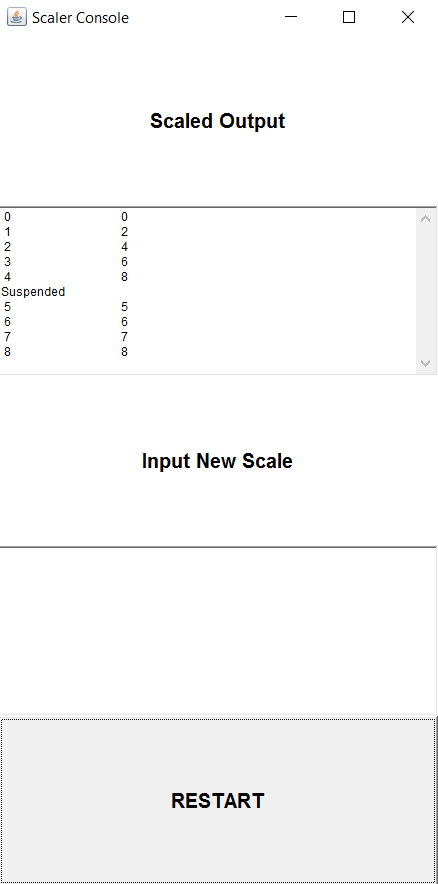
\includegraphics[width=2.5in]{uiSuspend}%
   		\label{fig_first_image}}
   	\hfil
   	\subfloat[Numbers have been Injected using the textbox.]{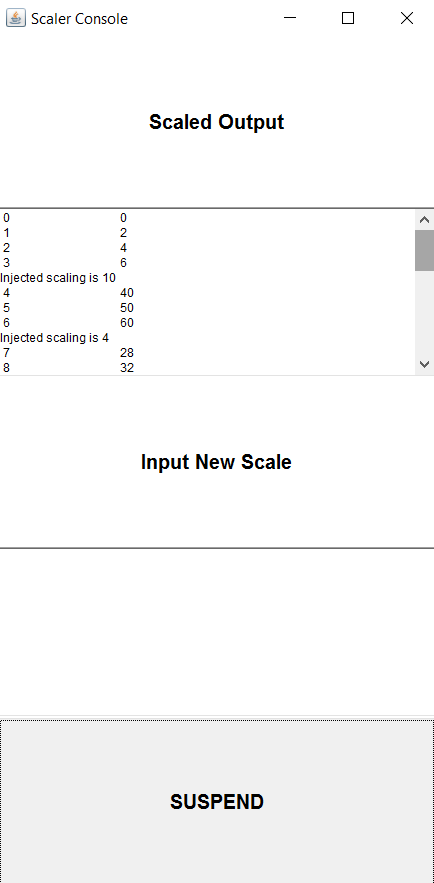
\includegraphics[width=2.5in]{uiInject}%
   		\label{fig_second_image}}
   	\caption{Output captures from the Scaler User Interface.}
   	\label{uiOut}
   \end{figure*}

   \subparagraph{Explanation} \hfill
   
   To implement the user interface, \textit{GConsole.groovy} was modified. In doing so, it removed the need for the controller process and the channels were redirected to the \textit{UserInterface.groovy} process as seen in figure \ref{fig:UI}. \textit{Scale.groovy} was also heavily modified to allow for the user to input values to inject into the system and for the button to suspend and resume scaling.
   
  
	
\end{document}
